\input{"../../../preamble"}

\begin{document}

\title{CSC263-Notes-01-21-2015}

\input{"../csc263-header"}
\rhead{January 21, 2015}

\section*{Lecture 06}

\subsection*{Dictionaries - \textit{Continued}}

\subsubsection*{Direct Mapping}

\noindent \begin{tabular}{| l | l | l | l | l | l | l |}
	\hline NL & 2 & NL & NL & 5 & $\ldots$ & 100 \\ \hline	
\end{tabular} \\
Search,delete,insert $\in \Theta(1)$, but space is an issue! space $\in O(n)$ where $n$ is the size of the keyspace

\subsubsection*{Hashing}

\begin{tabular}{| l | l | l | l | l | l | l | l | l | l |}
	\hline 9 & 4 & 7 & 5 & 5 & 2 & \textbf{8} & \textbf{5} & \textbf{6} & \textbf{7} \\ \hline
\end{tabular} \\

\noindent \begin{tabular}{| l | l | l | l | l | l | l | l | l | l |}
	\hline 9 & 7 & 9 & 8 & 6 & 5 & \textbf{8} & \textbf{5} & \textbf{6} & \textbf{7} \\ \hline
\end{tabular} 

\subsubsection*{Binary Search Trees}

\begin{itemize}
	\item for every node, all items in left subtree $\leq$ node.item $\leq$ all items in right subtree
	\item dictionary $S$ stores only $S.root$ (also $S.size$ usually)
	\item \texttt{TreeNode} has members \texttt{.item} (element stored in node), \texttt{.left} and \texttt{.right} (children)
\end{itemize} 

\begin{tabular}{| l | l | l | l | l | l | l |}
	\hline 5 & 7 & 2 & 0 & 20 & 4 & 9 \\ \hline
\end{tabular}

\begin{center}
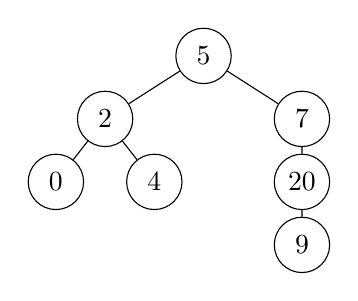
\begin{tikzpicture}[every node/.style={circle,draw,minimum size=2em,inner sep=1},
	baseline={(current bounding box.center)},
	level/.style={level distance=8mm,
	sibling distance=25mm/#1}]
\node {5} 
child {node {2}
	child {node {0}}
	child {node {4}}
	}
child {node {7}
	child {node {20}
		child {node {9}}
		}
	};
\end{tikzpicture}
\end{center}

\begin{lstlisting}[language=Python]
search(S,k):
	return treeSearch(S.root,k)

treeSearch(root, k):
	if root == NULL:
		# return null
		pass
	else if k < root.item.key:
		root = treeSearch(root.left, k)
	else if k > root.item.key:
		root = treeSearch(root.right, k)
	else:
		# k is root.item.key
		pass
	
	return root	
\end{lstlisting}

\newpage
\noindent insert 6:

\begin{center}
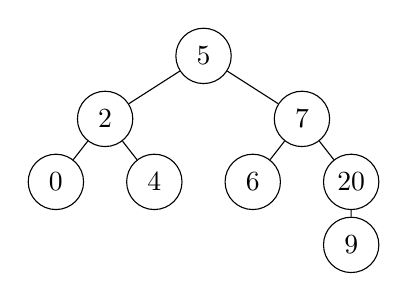
\begin{tikzpicture}[every node/.style={circle,draw,minimum size=2em,inner sep=1},
	baseline={(current bounding box.center)},
	level/.style={level distance=8mm,
	sibling distance=25mm/#1}]
\node {5} 
child {node {2}
	child {node {0}}
	child {node {4}}
	}
child {node {7}
	child {node {6}}
	child {node {20}
		child {node {9}}
		}
	};
\end{tikzpicture}
\end{center}

\begin{lstlisting}[language=Python]
insert(S,x):
	treeInsert(S.root, x)
	
treeInsert(root, x):
	if root == NULL:
		root = TreeNode(x)
	else if x.key < root.item.key:
		root.left = treeInsert(root.left, x)
	else if x.key > root.item.key:
		root.right = treeInsert(root.right, x)
	else
		# k is root.item.key
		
	return root
\end{lstlisting}

\newpage
\subsection*{\texttt{delete}}

\noindent If $x$ is not found $\rightarrow$ do nothing \\
If $x$ is found in a leaf $\rightarrow$ remove the leaf \\
If $x$ has only one sub-tree, remove $x$ and shift the subtree up to replace $x$ (splice around $x$) \\
If $x$ has two sub-trees:
\begin{itemize}
	\item it must have a \textit{successor} (the next node in the tree larger than $x$)
	\item the \textit{successor} must be the minimum node in the right subtree of $x$
	\item the \textit{minimum} is the left-most node in a tree
\end{itemize}

\begin{lstlisting}[language=Python,mathescape]
delete(S,x):
	S. root = treeDelete(S.root, x)
	
treeDelete(root, x):
	if root == NULL: # x.key not in $S \rightarrow$ should not happen!
		pass # nothing to remove
	else if x.key < root.item.key:
		root.left = treeDelete(root.left, x)
	else if x.key > root.item.key:
		root.right = treeDelete(root.right, x)
	else: # x.key == root.item.key
		# remove root.item
		if root.left == NULL or root.right == NULL:
			# root missing one child, replace with other child
			if root.left == NULL:
				root = root.right # NULL if both children are missing
			else:
				root = root.left
		else:
			# Root has two children: remove element w/ smallest key in
			# right subtree and move it to root
			return root.item, root.right = treeRemoveMini(root.right)
	return root

treeRemoveMini(root):
	# remove element w/ smallest key in root's subtree
	# return item and root of resulting subtree
	if root.left == NULL:
		# root stores item w/ smallest key; replace it w/ right child
		return root.item, root.right
	else:
		# left subtree not empty: root not the smallest
		item, root.left = treeRemoveMini(root.left)
		return item, root
\end{lstlisting}

\end{document}